\begin{figure}[H]
	\begin{subfigure}[c]{0.5\textwidth}
		\centering
		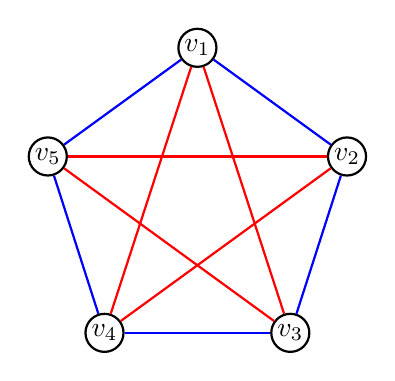
\begin{tikzpicture}
\tikzset{punkt/.style={circle, thick, draw=black, minimum width=0.2cm,inner sep=1}}
\node[punkt] at (0.0, 2.0) (a) {$v_1$};
\node[punkt] at (1.9, 0.62) (b) {$v_2$};
\node[punkt] at (1.18, -1.62) (c) {$v_3$};
\node[punkt] at (-1.18, -1.62) (d) {$v_4$};
\node[punkt] at (-1.9, 0.62) (e) {$v_5$};
			\draw [thick, draw=blue] (a) -- (b);
			\draw [thick, draw=blue] (b) -- (c);
			\draw [thick, draw=blue] (c) -- (d);
			\draw [thick, draw=blue] (d) -- (e);
			\draw [thick, draw=blue] (e) -- (a);

			% Red edges
			\draw [thick, draw=red] (a) -- (c);
			\draw [thick, draw=red] (a) -- (d);
			\draw [thick, draw=red] (b) -- (d);
			\draw [thick, draw=red] (b) -- (e);
			\draw [thick, draw=red] (c) -- (e);
		\end{tikzpicture}
		\caption{A $2$-edge coloring $\chi$ on $K_{v}$}
	\end{subfigure}
	\begin{subfigure}[c]{0.5\textwidth}
		\centering
		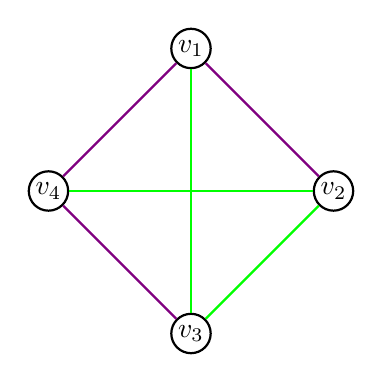
\begin{tikzpicture}
			\tikzset{punkt/.style={circle, thick, draw=black, minimum width=0.5cm,inner sep=1}}

\node[punkt] at (0.0, 1.81) (a) {$v_1$};
\node[punkt] at (1.81, 0.0) (b) {$v_2$};
\node[punkt] at (0.0, -1.81) (c) {$v_3$};
\node[punkt] at (-1.81, -0.0) (d) {$v_4$};
			\draw [thick, violet] (a) -- (d);
			\draw [thick, draw=violet] (a) -- (b);
			\draw [thick, draw=violet] (c) -- (d);
			\draw [thick, draw=green] (b) -- (d);
			\draw [thick, draw=green] (b) -- (c);
			\draw [thick, draw=green] (a) -- (c);
		\end{tikzpicture}
		\caption{A $2$-edge coloring $\gamma$ on $K_{u}$}
	\end{subfigure}
	\caption{Two 2-edge colorings which admits no monochromatic cliques of order $3$.}
	\label{fig:blow_up_1}
\end{figure}
